\documentclass{article}

% Language setting
\usepackage[italian]{babel}

% Set page size and margins
% Replace `letterpaper' with `a4paper' for UK/EU standard size
\usepackage[a4paper,top=2cm,bottom=2cm,left=2cm,right=2cm,marginparwidth=1.75cm]{geometry}

\usepackage[utf8]{inputenc}
\usepackage[T1]{fontenc}
\usepackage{lmodern}

% Useful packages
\usepackage{matlab-prettifier} % per il codice Matlab colorato carino
\usepackage{csvsimple-l3} % per le tabelle
\usepackage{booktabs} % per le tabelle
\usepackage{longtable} % per le tabelle
\usepackage{amsmath}
\usepackage{amsfonts}
\usepackage[thinc]{esdiff}
\usepackage{minted}
\usepackage{bbm}
\usepackage{bm}
\usepackage{optidef}
\usepackage{graphicx}
\usepackage[colorlinks=true, allcolors=blue]{hyperref}
\usepackage{subcaption}   % Per immagini affiancate con didascalie


\title{Report NO4LSP}
\author{Chiodo Martina - 343310 \\ Vigè Sophie - 339268}
\date{}

\begin{document}
%\begin{titlepage}
    \newgeometry{left=1cm, right=1cm, top=3cm, bottom=3.5cm}  % Margini specifici per questa pagina
    
    \begin{center}
    
\includegraphics[width=0.35\textwidth]{img/logo_polito_2021.jpg}\\[1cm] 
    {\huge POLITECNICO DI TORINO}\\[1.5cm]
    \textbf{Corso di Laurea\\in Ingegneria Matematica}\\[3cm]
    
     
    {\huge Report NO4LSCP}\\[1cm]
    {\large Chiodo Martina - 343310 \\
    Vigè Sophie - 339268}
    
    
    
    \vfill
    
    Anno Accademico 2024-2025
    \end{center}
    
    \restoregeometry
    
    \end{titlepage}

\maketitle

\section*{INTRODUZIONE}
This assignment aims to evaluate and compare the results of two numerical methods for unconstrained optimization applied to various problems.
The method we decided to implement are the Nealder Mead method and the Modified Newton method. In particular for each problem we are going to run $11$ experiments for both methods, the first one is run with a given initial point and the others with perturbations of it. These experiments will contribute to compute some statistics that will help us to compare the method, such as the minimum value found, the number of successful runs, the number of iterations needed by the method to converge and the experimental rate of convergence.

We can now proceed giving some details on how the algorithms have been implemented.

\subsection*{Nealder Mead Method}
The Nelder-Mead Method is a derivative-free optimization technique that minimizes the objective function by evaluating it at the vertices of a simplex, which it uses to navigate the multidimensional space.
The method employs four main operations: reflection, expansion, contraction, and shrinking, each of them is controlled by a parameter $\rho$ for reflection, $\chi$ for expansion, $\gamma$ for contraction, and $\sigma$ for shrinking. These parameters are provided as inputs to the algorithm to optimize performance for each specific problem.

The initial simplex is constructed by perturbing the initial point, as we are not given an initial simplex. Specifically, the $i^{th}$ vertex is generated by perturbing one component of the initial point, formulated as $x_{i} = x_0 + a e_i$. These perturbations are not fixed; for each vertex, we evaluate few values of $a$ in order to minimize the objective function computed in $x_i$, aiming to get closer to the minimum point and obtaining a faster convergence to it.

The stopping criterion for the method is based on the tolerance of the current simplex size. Ideally, the simplex shrinks as it approaches the minimum, so once the simplex has significantly reduced in size, we consider the method to have converged.

This algorithm is heuristic, meaning that convergence to a global minimum is not guaranteed, as it may get stuck in a non-stationary point.


\subsection*{Modified Newton Method}
The second method we have implemented is the Modified Newton Method, which leverages the gradient and the Hessian matrix of the function to move along descent directions at each iteration to reach the minimum.

This method faces two main challenges: performing an efficient line search at each iteration and ensuring the Hessian matrix is positive definite to compute the descent direction.

To address the first issue, we use a backtracking strategy for the line search. The parameters for the Armijo conditions and the maximum number of backtracking steps varies for each problem to optimize performance.

For the second issue, we regularize the Hessian matrix by adding a positive quantity to its diagonal until it becomes positive definite. We determine the positive definiteness by attempting a Cholesky factorization, which, if successful, is also used to solve the linear system to find the descent direction.

The stopping criterion is bases on the tolerance of the norm of the gradient.


\subsection*{Rate of Convergence}
As said before, a way to evaluate the performance of a numerical method is to compute the rate of convergence. In some cases, this could not be possible because in its definition appears the minimum of the found which is not known a priori.
Then what we will compute is the experimental rate of convergence which is defined as 
\begin{equation}
    q \approx \frac{ \log \left(\frac{\| \hat{e}^{(k+1)} \|}{\| \hat{e}^{(k)} \|} \right)}{ \log \left(\frac{\| \hat{e}^{(k)} \|}{\| \hat{e}^{(k-1)} \|} \right)}
    \quad \text{ for $k$ large enough}
    \label{definizione_roc}
\end{equation}
where $\hat{e}^{(k)} = x^{(k)} - x^{(k-1)}$ approximates the error at the $k$-th iteration (if the exact solution is unknown).
This approximation is valid for $k$ large enough, so it is possible that the value we compute may not be entirely reliable.


\newpage
\section*{PROBLEMA 64}
\input{chap/pb64.tex}

\newpage
\section*{PROBLEMA 75}
\subsection*{Model}
The function described in this problem is the following 
\begin{equation*}
\begin{aligned}
    &F(\boldsymbol{x}) = \frac{1}{2}\sum_{k=1}^n f_k^2(\boldsymbol{x}) \\
    &f_k(\boldsymbol{x}) = x_k-1, & k=1 \\
    &f_k(\boldsymbol{x}) = 10(k-1)(x_k - x_{k-1})^2, & 1<k\leq n
\end{aligned}
\end{equation*}
where $n$ is the length of the input vector $\boldsymbol{x}$.
With the given starting point for minimization being 
\[\boldsymbol{x_0}=[-1.2,-1.2,...,-1.2,-1]' \in \mathbbm{R}^n.\]
The gradient of $F(\boldsymbol{x})$ is the following (note that, besides the first and last components, all the others have the same structure).
\begin{equation*}
    \nabla F(\mathbf{x}) = 
    \begin{bmatrix}
        \frac{\partial F}{\partial x_1}(\mathbf{\boldsymbol{x}}) \\
        \vdots \\
        \frac{\partial F}{\partial x_k}(\mathbf{\boldsymbol{x}}) \\
        \vdots \\
        \frac{\partial F}{\partial x_n}(\mathbf{\boldsymbol{x}})
    \end{bmatrix}
    =
    \begin{bmatrix}
        \frac{\partial }{\partial x_1}\frac{1}{2}(f_1^2+f_2^2)(\boldsymbol{x}) \\
        \vdots \\
        \frac{\partial F}{\partial x_k}\frac{1}{2}(f_k^2+f_{k+1}^2)(\boldsymbol{x}) \\
        \vdots \\
        \frac{\partial F}{\partial x_n}\frac{1}{2}f_n^2(\boldsymbol{x})
    \end{bmatrix}
    =
    \begin{bmatrix}
        x_1-1-200\cdot (x_2-x_1)^3 \\
        \vdots \\
        200 \cdot \Big((k-1)^2(x_k-x_{k-1})^3-k^2(x_{k+1}-x_k)^3\Big)\\
        \vdots \\
        200 \cdot (n-1)^2(x_n-x_{n-1})^3
    \end{bmatrix}
\end{equation*}
The Hessian matrix of $F(\boldsymbol{x})$ is sparse since only on three diagonals elements different from zeros are present. They are the following:
\begin{align*}
    \frac{\partial^2 F}{\partial x_1^2} (\boldsymbol{x}) &= 1+600\cdot(x_2-x_1)^2 \\
    \frac{\partial^2 F}{\partial x_k^2} (\boldsymbol{x}) &= 600\cdot\Big((k-1)^2(x_k-x_{k-1})^2+k^2(x_{k+1}-x_k)^2 \Big), \quad 1 < k < n  & \\
    \frac{\partial^2 F}{\partial x_n^2} (\boldsymbol{x}) &=600\cdot(n-1)^2(x_n-x_{n-1})^2 \\
    \frac{\partial^2 F}{\partial x_k \partial x_{k-1}} (\boldsymbol{x}) &= -600\cdot (k-1)^2(x_k-x_{k-1})^2, \quad 1<k\leq n.
\end{align*}
It is easy to notice that $F$, being the sum of squared functions, is always non negative. Furthermore, $F(\boldsymbol{x})=0$ if and only if $\boldsymbol{x}=[1,1,...,1]'$ since $f_1(\boldsymbol{x})^2=0$ if and only if $x_1=1$ and, for every $1<k\leq n$, $f_k(\boldsymbol{x})=0$ if and only if $x_k=x_{k-1}$.

More formally, we can see that $\boldsymbol{x}=[1,1,...,1]'$ solves the equation $\nabla F(\boldsymbol{x})=\boldsymbol{0}$. Since $F$ is convex (being the sum of convex functions) and differentiable, we know that any stationary point is a global minimum point for $F$. 

Then $\boldsymbol{x}=[1,1,...,1]'$ is the only global minimum point for $F$.

We plot the function for $n=2$ in a neighborhood of the minimum point.
\begin{figure}[H]
    \centering
    \begin{subfigure}{0.45\textwidth}
        \centering
        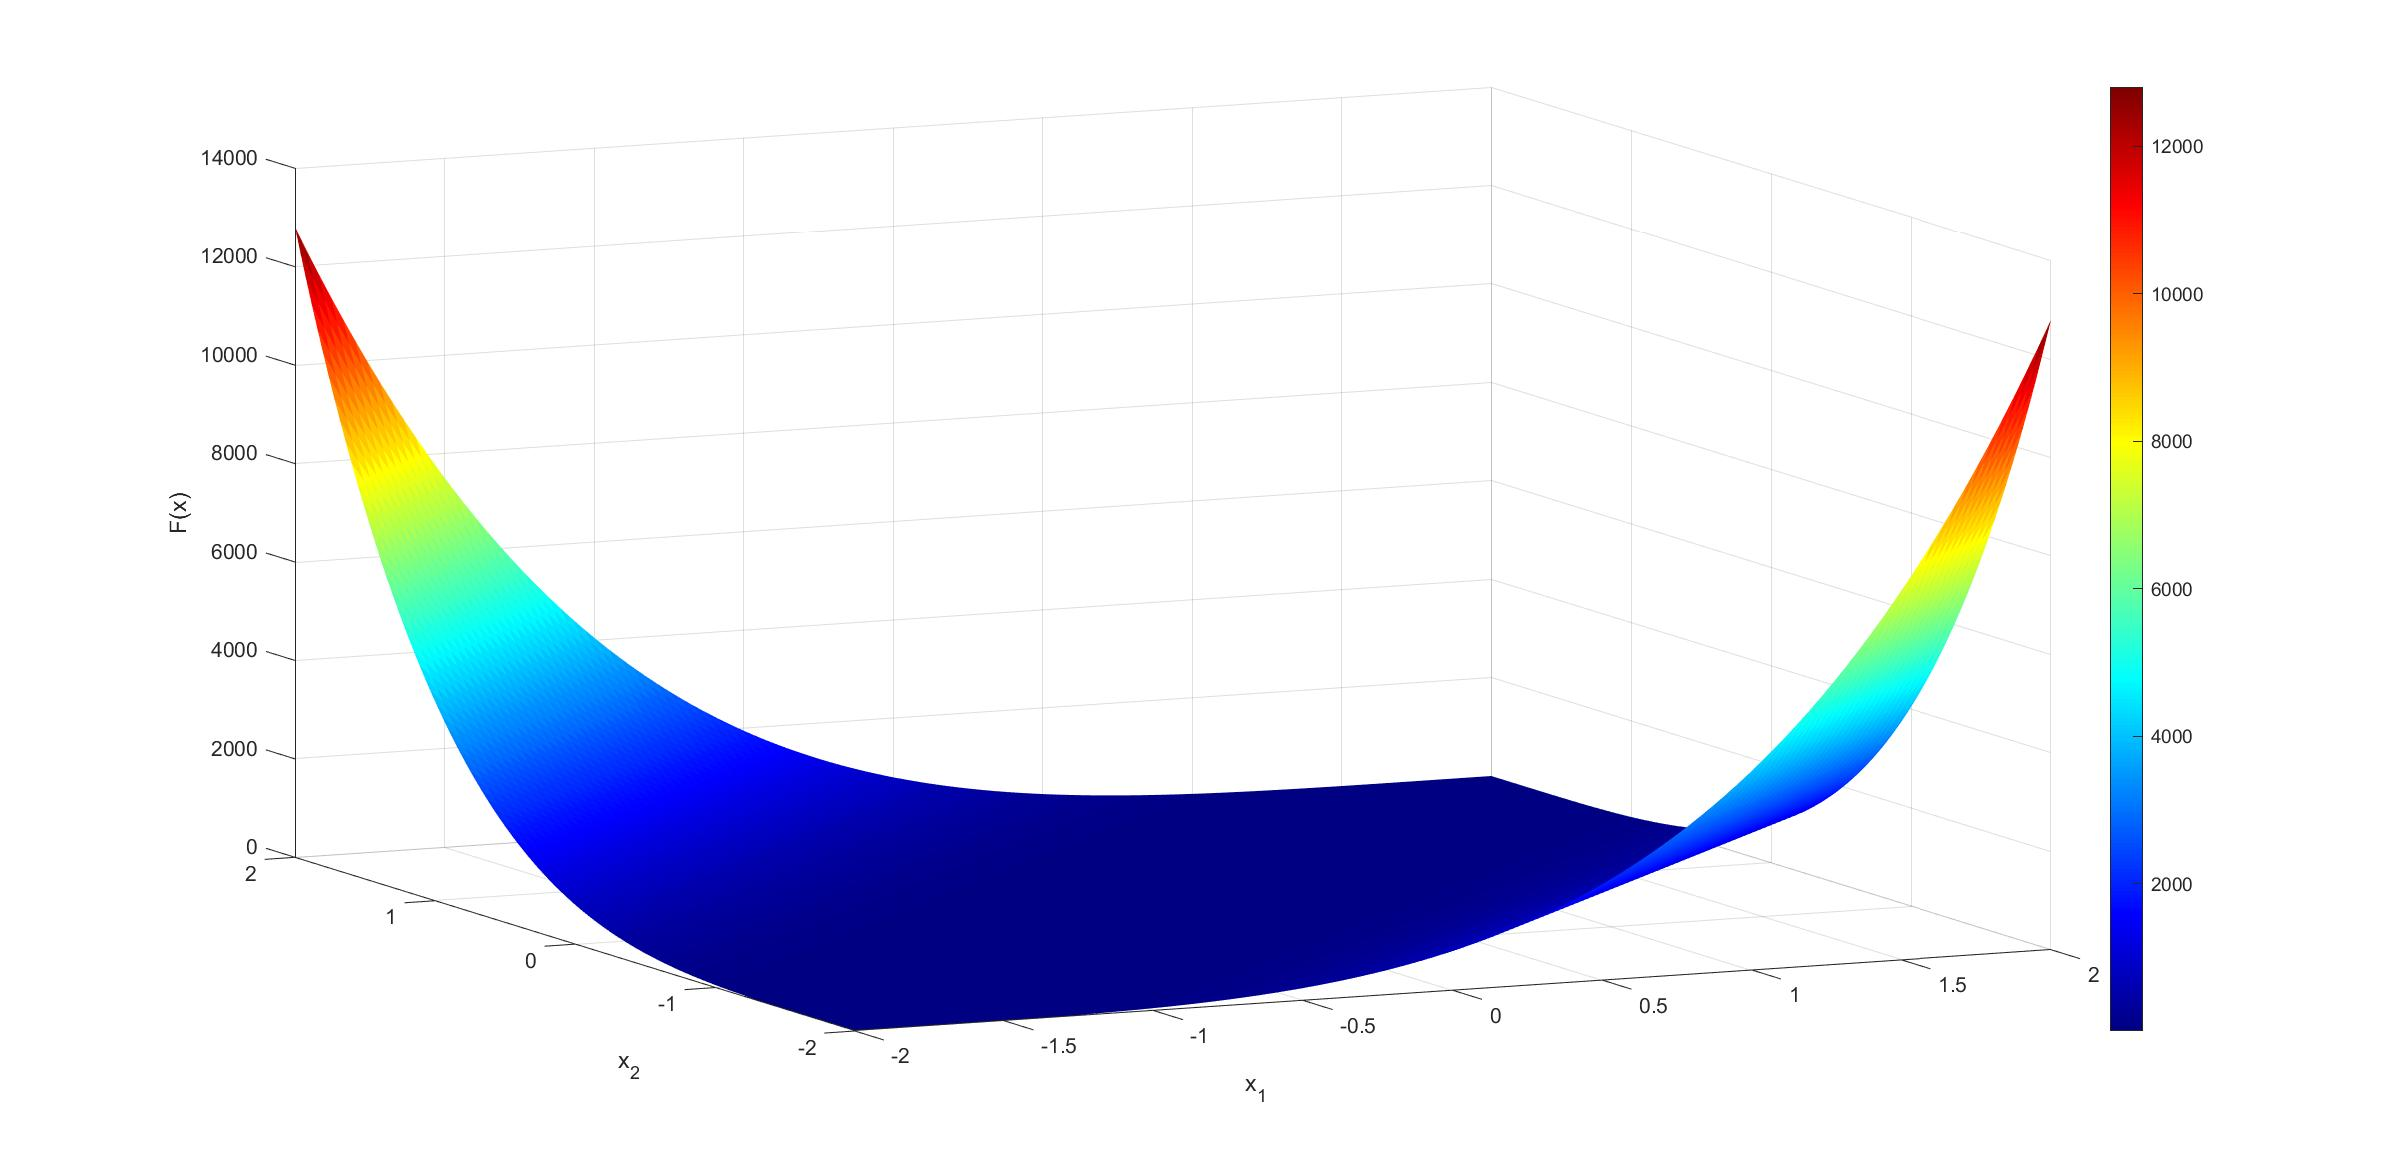
\includegraphics[width=\textwidth]{img/function_pb75_angolo1.jpg}
        \caption{}
    \end{subfigure}
    \begin{subfigure}{0.45\textwidth}
        \centering
        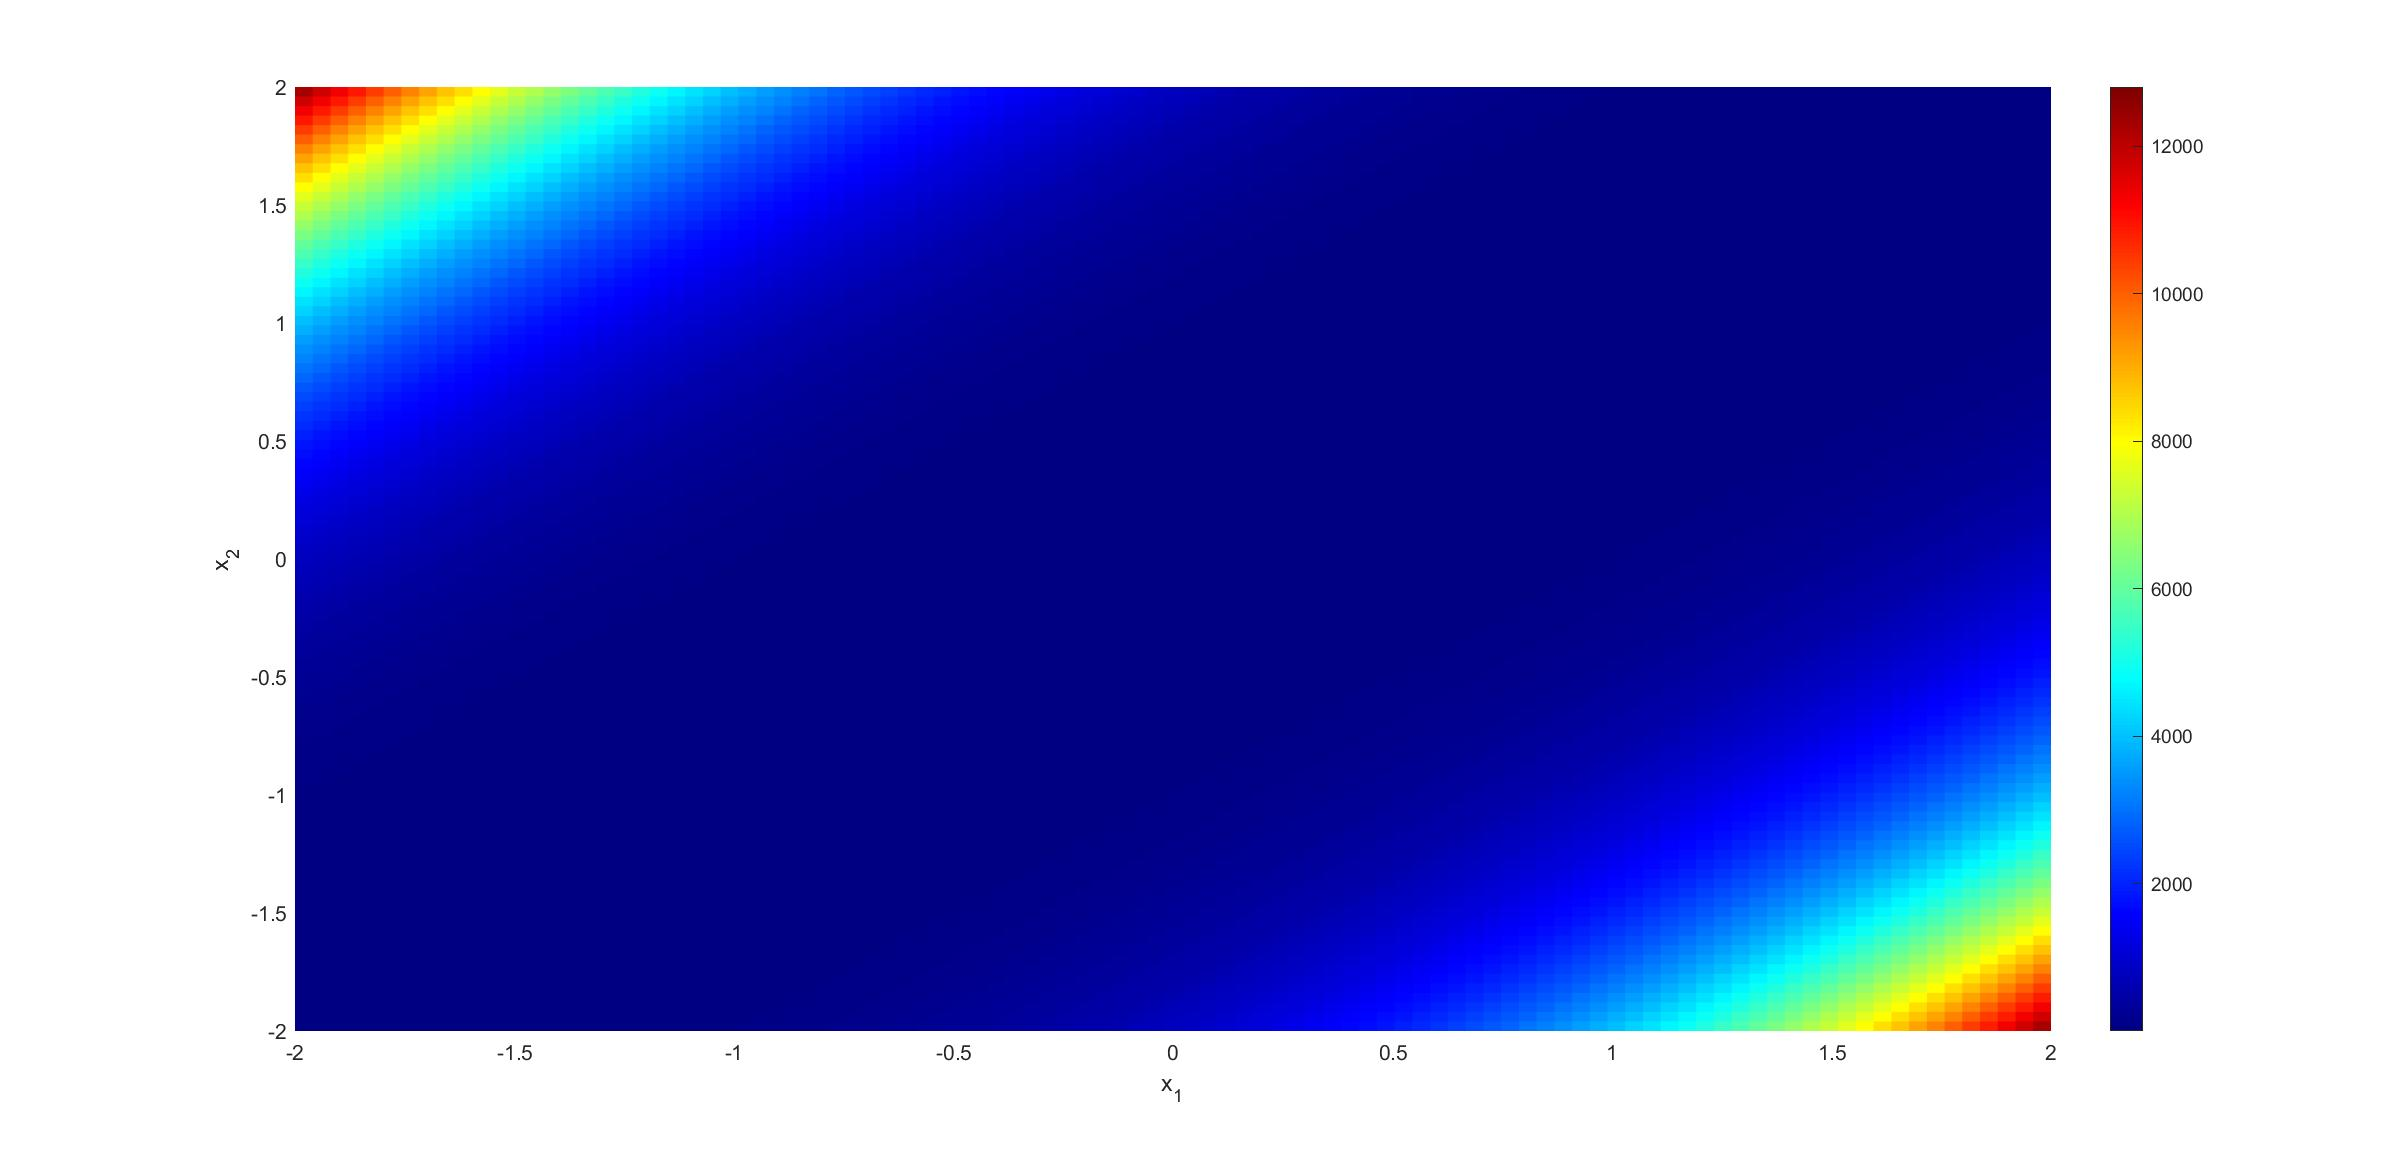
\includegraphics[width=\textwidth]{img/function_pb75_angolo2.jpg}
        \caption{}
    \end{subfigure}
    \caption{function $F(\boldsymbol{x})$ for $n=2$}
%\label{fig:funzione 2D pb 75}
\end{figure}
We can easily see that the central area, where the minimum point is located,
is quite flat. This means that the minimization methods used might have some troubles
when reaching this area because they might get stuck before reaching the minimizer.

\subsection*{Nelder Mead Method}
We runned the minimisation problem with Nelder Mead method using the following parameters:
\begin{eqnarray*}
    \text{reflection } \rho &=& 1.1 \\
    \text{expansion } \chi &=& 2.5 \\
    \text{contraction } \gamma &=& 0.6 \\
    \text{shrinking } \sigma &=& 0.5.
\end{eqnarray*}
The aim, with this choice, is to try to keep the simplex big enough so that
the method will not get stuck too easily in the almost flat areas of the function's graph.

We now report a table summarizing the results obtained by running the Nelder-Mead method
on the considered problem for dimensions $n=$10, 25, 50 and for a total of 11 starting 
points for each dimension, obtained as perturbations of the given one.

\begin{figure}[H]
    \centering
    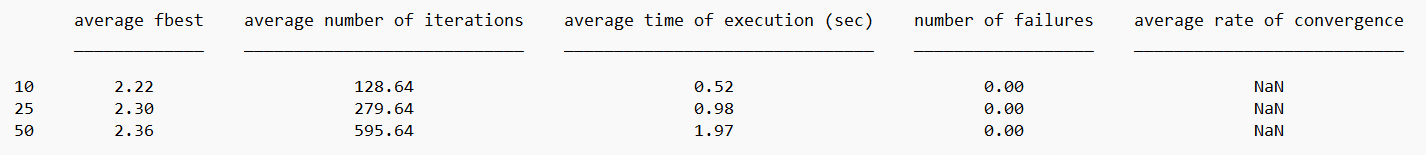
\includegraphics[width=1\textwidth]{img/pb75_table_SX.png}
    \caption{Results obtained by running the Nelder Mead method on problem 75.} 
    \label{pb 75 table SX}
\end{figure}

We notice that the method reports zero failures, which means that it never stopped because of the maximum 
number of iterations allowed (in this case $200\cdot n$) had been reached. However, the best value of the 
function $F$ that has been found is not so close to the expected value (which as observed before should be 0).
The problem is in the starting point. In fact, even with the random perturbations, it always falls in the flat area 
of the function. Tuning the parameters in a way that encourages the expansion of the simplex's area is not enough 
to prevent the method from getting stuck here. It can be seen that, if we use as a staring point for example $[0,0,...,0]'$, 
the results are a bit closer to the exact one (around 0.35). 

The Nelder Mead method does not guarantee convergence and it is sensitive to the starting point and this becomes evident 
in this optimisation problem.

Concerning the rate of convergence, the fact that \verb+Nan+ is always reported is due to the construction of the method
itself. In fact not necessarily at every iteration the best point of the current simplex is updated; expecially when contraction
and shrinking phases are reached, it means that new promising points were not found, so it is quite likely that the current best point
does not change among consecutive iterations. This is a problem when it comes to apply the formula for the experimental rate of 
convergence $\eqref{definizione_roc}$, since it leads the denominator to be 0.

\medskip
\subsection*{Modified Newton Method - Exact Derivatives}
As previously shown, we can easily compute the exact derivatives for the gradient and the Hessian matrix of $F(x)$. The Hessian should be stored
as a sparse matrix due to its large dimension. We can then apply the Modified Newton Method to the considered problem, obtaining the following 
results. 
\begin{figure}[H]
    \centering
    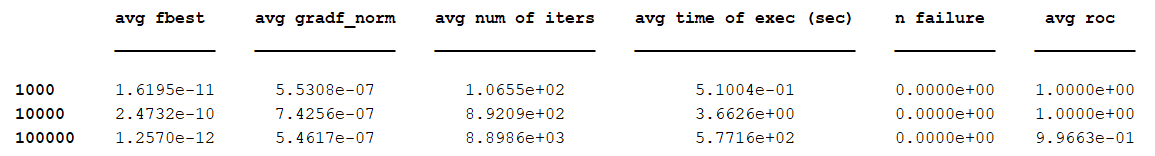
\includegraphics[width=1\textwidth]{img/pb75_table_MN.png}
    \caption{Results obtained by running the Modified Newton method on problem 75 using exact derivatives.} 
    \label{pb 75 table MN}
\end{figure}
As expected, this method is performing much better due to the exploitation of the information contained in the gradient and the Hessian. 
In every tested dimension $n$ it reaches the exact solution within the maximum number of iterations fixed for the corresponding dimension
(in this case $n$ has been used). For the others parameters the following values have been used:
\begin{itemize}
    \item tolerance for the norm of the gradient: $10^{-6}$ for every dimension
    \item parameter $\rho \in (0,1)$ for the reduction of the steplength in backtracking: $\rho$= 
    $\begin{cases}
        0.4 \quad n=10^3 \\
        0.3 \quad n=10^4 \\
        0.4 \quad n=10^5
    \end{cases}$
    \item parameter $c_1 \in (0,1)$ for the Armijo condition: $c_1$= 
    $\begin{cases}
        10^{-4} \quad n=10^3 \\
        10^{-4} \quad n=10^4 \\
        10^{-3} \quad n=10^5
    \end{cases}$
    \item maximum number of backtracking steps allowed: \texttt{btmax} = 
    $\begin{cases}
        36 \quad n=10^3 \\
        28 \quad n=10^4 \\
        36 \quad n=10^5
    \end{cases}$ 
\end{itemize}
The values of $\rho$ and \texttt{btmax} for every dimension has been chosen in such a way that stagnation is not allowed. 
In fact $\rho^{\texttt{btmax}}>\epsilon_m$, where the machine precision is $\epsilon_m \approx 10^{-16}$.

That experimental rate of convergence is approximately 1, so we are losing some of the strength of pure Newton method. 

In the following figure we can see two examples of the progress of the minimum value of $F(x)$.
\begin{figure}[htbp]
    \centering
    % Prima immagine
    \begin{subfigure}[t]{0.45\textwidth}  % Larghezza del 45% del testo
        \centering
        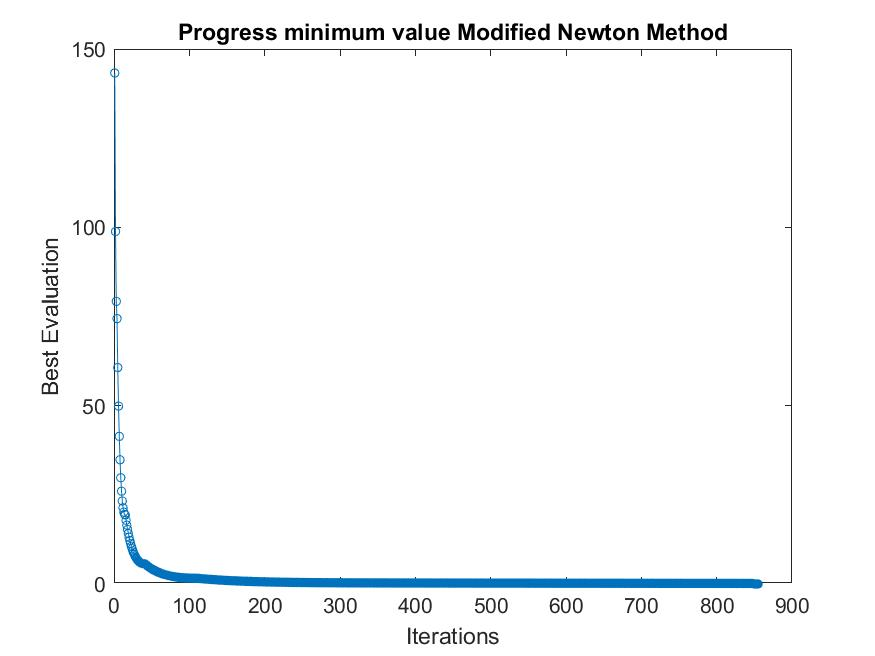
\includegraphics[width=\textwidth]{img/pb75_1e3_MN_convergence.jpg}
        \caption{$n=10^3$}
    \end{subfigure}
    \hspace{1cm} %spaziatura tra le immagini
    % Seconda immagine
    \begin{subfigure}[t]{0.45\textwidth}
        \centering
        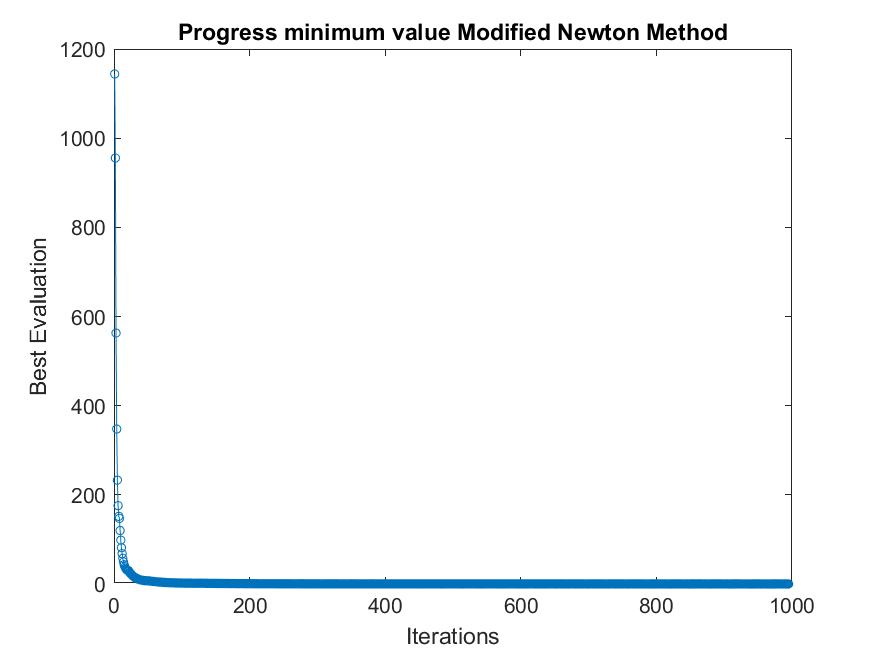
\includegraphics[width=\textwidth]{img/pb75_1e4_MN_convergence.jpg}
        \caption{$n=10^4$}
    \end{subfigure}
    % Didascalia generale
    \caption{Example of convergence to zero of the value of $F(x)$.}
    \label{convergenze MN 75}
\end{figure}
Notice how fast it decreases in the first iterations, while the convergence becomes smaller when entering the almost flat area of the function.

\medskip
\subsection*{Modified Newton Method - Approximated Derivatives}
Let us now analyze what happens if we suppose not to be able to compute the exact derivatives of function $F$.

Using forward difference with step $h_k$ (where $h_k$ can either be constant or $h_k=h|\hat{x}_k|$ where $k=1,...,n$ and $\hat{x}$ is the point 
where the approximation is calculated), we can obtain an approximation of the gradient of $F$. We denote as $\vec{e_k} \in \mathbbm{R}^n$ the k-th vector of the canonic basis. 
Note that we can exploit the structure of the function
in order to avoid the evaluation of the whole $F$. This makes the evaluation much faster.
\begin{eqnarray*}
    \frac{\partial F}{\partial x_k}(x) &\approx& \frac{F(x+h_k \vec{e_k})-F(x)}{h_k} 
    = \frac{f_k^2(x+h_k \vec{e_k}) +f_{k+1}^2(x+h_k\vec{e_k}) -f_k^2(x) -f_{k+1}^2(x) }{2h_k} \quad 1\leq k<n \\
    \frac{\partial F}{\partial x_n}(x) &\approx& \frac{f_n^2(x+h_n\vec{e_n}) - f_n^2(x)}{2h_n}.
\end{eqnarray*}
The same reasoning can be applied to approximate the Hessian using the general formula 
$$\frac{\partial^2 f}{\partial x_i \partial x_j} (x) \approx \frac{f(x+h_i\vec{e_i}+h_j\vec{e_j}) - f(x+h_i\vec{e_i}) - f(x+h_j\vec{e_j}) + f(x) }{h_ih_j}$$
and recalling that each $f_k$ for $1<k\leq n$ only depends on $x_k$ ad $x_{k-1}$. We obtain the following 
\begin{eqnarray*}
    \frac{\partial^2 F}{\partial x_k^2} &\approx& \frac{f_k^2(x+2h_k\vec{e_k}) + f_{k+1}^2(x+2h_k\vec{e_k}) -2f_k^2(x+h_k\vec{e_k}) -2f_{k+1}^2(x+h_k\vec{e_k}) +f_k^2(x) + f_{k+1}^2(x) }{2h_k^2}, \quad 1 \leq k <n \\
    \frac{\partial^2 F}{\partial x_n^2} &\approx& \frac{f_n^2(x+2h_n\vec{e_n}) - 2f_n^2(x+h_n\vec{e_n} + f_n^2(x)) }{2h_n^2} \\
    \frac{\partial^2 F}{\partial x_k \partial x_{k-1}} &\approx& \frac{f_k^2(x+h_k\vec{e_k}+h_{k-1}\vec{e_{k-1}}) + f_{k+1}^2(x+h_k\vec{e_k}) -f_k^2(x+h_k\vec{e_k}) -f_{k+1}^2(x+h_k\vec{e_k})}{2h_k h_{k-1}} + \\
    && + \frac{ -f_k^2(x+h_{k-1}\vec{e_{k-1}}) -f_{k+1}^2(x) +f_k^2(x) + f_{k+1}^2(x) }{2h_k h_{k-1}}, \quad 1<k<n \\
    \frac{\partial^2 F}{\partial x_n \partial x_{n-1}} &\approx& \frac{f_n^2(x+h_n\vec{e_n}+h_{n-1}\vec{e_{n-1}}) -f_n^2(x+h_n\vec{e_n}) -f_n^2(x+h_{n-1}\vec{e_{n-1}}) +f_n^2(x) }{2h_n h_{n-1}}
\end{eqnarray*}
These are the only elements we have to compute to approximate the Hessian, since it is tridiagonal and we exploit its simmetry to avoid computing 
the elements of the upper diagonal.


\newpage
\section*{PROBLEMA 76}
\subsection*{Model}
The function described in this problem is the following
\begin{equation*}
    \begin{aligned}
    & F(\mathbf{x}) = \frac{1}{2} \sum_{k=1}^{n} f_k^2(x) \\
    & f_k(\mathbf{x}) = x_k - \frac{x_{k+1}^2}{10}, \quad   1 \leq k < n \\   
    & f_n(\mathbf{x}) = x_n - \frac{x_1^2}{10}
    \end{aligned}
\end{equation*}
where $n$ denotes the dimensionality of the input vector $\mathbf{x}$.
\\ The starting point for the minimization is the vector $\mathbf{x}_0 = [2, 2, \ldots, 2]$.


To be able to say something more about the behaviour of the problem is useful to look at the gradient of the function $F(\mathbf{x})$ and at its Hessian matrix.
\begin{equation*}
    \nabla F(\mathbf{x}) = 
    \begin{bmatrix}
        \frac{\partial F}{\partial x_1}(\mathbf{x}) \\
        \vdots \\
        \frac{\partial F}{\partial x_k}(\mathbf{x}) \\
        \vdots \\
        \frac{\partial F}{\partial x_n}(\mathbf{x})
    \end{bmatrix}
    =
    \begin{bmatrix}
        \frac{\partial}{\partial x_1} \frac{1}{2}\left[f_n^2 + f_1^2\right] (\mathbf{x})\\
        \vdots \\
        \frac{\partial}{\partial x_k} \frac{1}{2}\left[f_{k-1}^2 + f_k^2\right] (\mathbf{x})\\
        \vdots \\
        \frac{\partial}{\partial x_n}  \frac{1}{2}\left[f_{n-1}^2 + f_n^2\right] (\mathbf{x})
    \end{bmatrix}
    =
    \begin{bmatrix}
        -\frac{x_1}{5}\left(x_n - \frac{x_1^2}{10}\right) + \left(x_1 - \frac{x_1^2}{10}\right) \\
        \vdots \\
        -\frac{x_k}{5}\left(x_{k-1} - \frac{x_k^2}{10}\right) + \left(x_k - \frac{x_{k+1}^2}{10}\right) \\
        \vdots \\
        -\frac{x_n}{5}\left(x_{n-1} - \frac{x_n^2}{10}\right) + \left(x_n - \frac{x_1^2}{10}\right)
    \end{bmatrix}
\end{equation*}
Due to the particular structure of the function, the Hessian matrix as a sparse structure, with only 3 diagonals different from zero. The non-zero elements are the following:
\begin{align*}
    \frac{\partial^2 F}{\partial x_k^2} (\mathbf{x}) &= -\frac{1}{5}x_{k-1} - \frac{3}{50}x_k^2  + 1, \quad 1 < k \leq n  &
    \frac{\partial^2 F}{\partial x_1^2} (\mathbf{x}) &= -\frac{1}{5}x_{n} - \frac{3}{50}x_1^2  + 1, \\
    \frac{\partial^2 F}{\partial x_k \partial x_{k+1}} (\mathbf{x}) &= -\frac{1}{5}x_{k+1}, \quad 1 \leq k < n  &
    \frac{\partial^2 F}{\partial x_n \partial x_1}(\mathbf{x}) &= -\frac{1}{5}x_1  \\
    \frac{\partial^2 F}{\partial x_k \partial x_{k-1}}(\mathbf{x}) &= -\frac{1}{5}x_{k}, \quad 1 < k \leq n  &
    \frac{\partial^2 F}{\partial x_1 \partial x_{n}}(\mathbf{x}) &= -\frac{1}{5}x_{n}
\end{align*}
We can now easily notice that the gradient of the function is null when all the components of the vector $\mathbf{x}$ are equal to 0, in this case the Hessian matrix is positive definite, so the point $\mathbf{x} = \mathbf{0}$ is a minimum of the function $F(\mathbf{x})$. 
Because of the definition of the function, $0$ is the lowest value the function can assume, so the minimum found is global.


\medskip
\subsection*{Nealder Mead Method}
We now report a table containing some general results obtained by running the Nealder Mead method on the function $F(\mathbf{x})$.

\begin{figure*}[htbp]
    \centering
    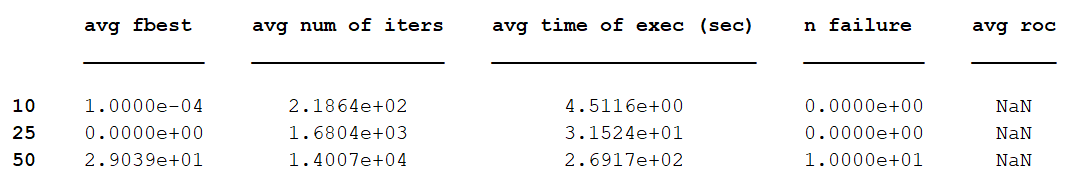
\includegraphics[width = 0.9\textwidth]{img/pb76_table_SX.png}
    \caption{Resultats obtained by running the symplex method on the problem $76$.}
\end{figure*}

First thing we can notice is that for smaller dimensionalities the symplex method is able to find the minimum in a reasonable amount of time, but when the dimensionality becomes higher the method starts failing.
From the plot in figure $\eqref{fig:iter}$, we can see that for most points belonging to $\mathbb{R}^{50}$, the method keeps iterating until the maximum number of iterations is reached without satisfying the stopping criterion.
This behaviour can probably be explained by the fact that when the dimensionality increases the starting point is more far from the minimum due to its definition, so the method needs to perform more iterations to reach the minimum.
\begin{figure}[htbp]
    \centering
    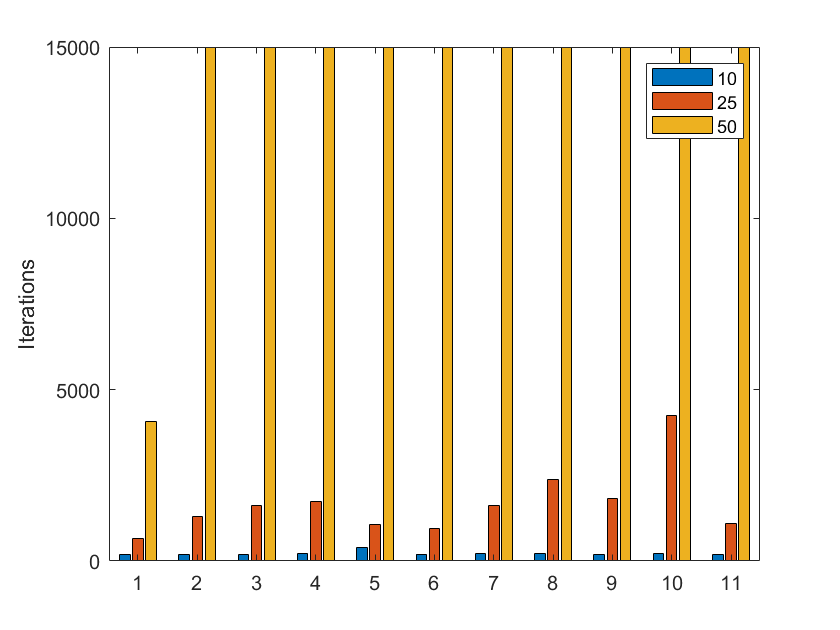
\includegraphics[width = 0.5\textwidth]{img/pb76_SX_iter.png}
    \caption{Number of iterations needed by the Nealder Mead method to find the minimum of the problem $76$ for each starting point.}
    \label{fig:iter}
\end{figure}

From the previous table, we can notice that the experimental rate of convergnce is always \verb+Nan+: this is due to the fact that in the last iterations the value of $\mathbf{x}^{(k)}$ does not change much and thus it yields a division by zero in the formula $\eqref{definizione_roc}$ which defines the experimental rate of convergence.
This can be seen in the following plots, showing that, in the last iterations, the approximated value of the minimum seems to be stationary.
\begin{figure}[htbp]
    \centering
    % Prima immagine
    \begin{subfigure}[t]{0.35\textwidth}  % Larghezza del 45% del testo
        \centering
        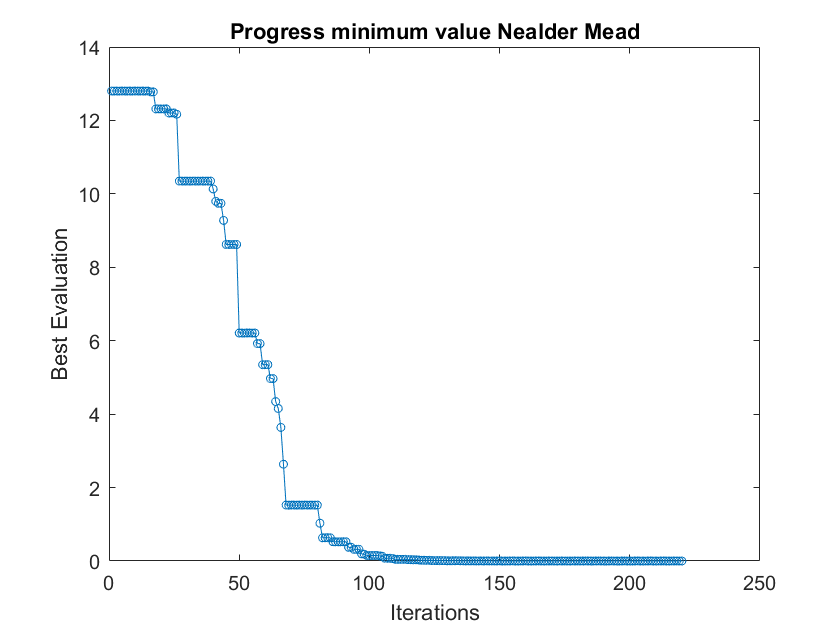
\includegraphics[width=\textwidth]{img/pb76_SX_es10.png}
        \caption{dimension $10$}
        \label{fig:R6}
    \end{subfigure}
    \hspace{1cm} %spaziatura tra le immagini
    % Seconda immagine
    \begin{subfigure}[t]{0.35\textwidth}
        \centering
        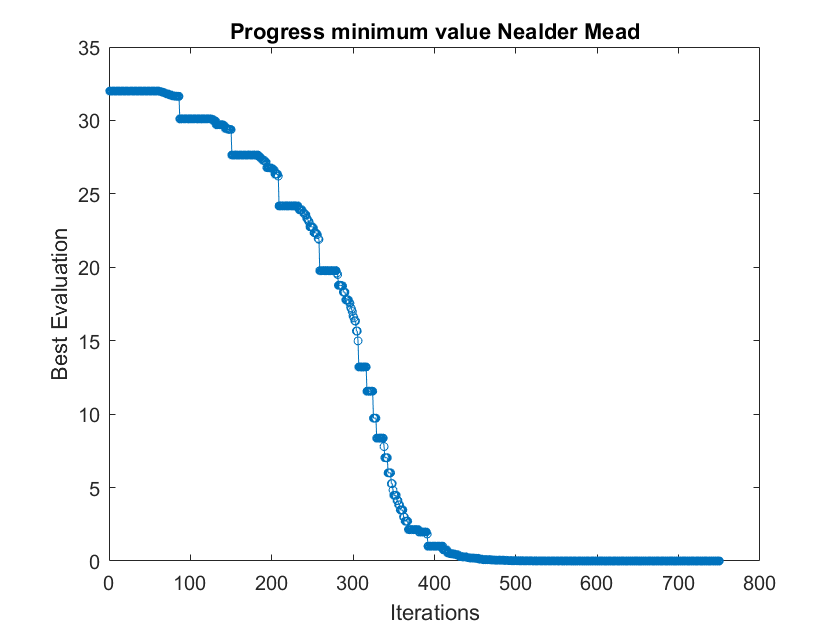
\includegraphics[width=\textwidth]{img/pb76_SX_es25.png}
        \caption{dimension $25$}
        \label{fig:R8}
    \end{subfigure}
    % Didascalia generale
    \caption{ \small Plots of the progresses of the Nealder Mead method for different dimensionalities for the problem $76$.}
    \label{fig:overall}
\end{figure}


\medskip
\subsection*{Modified Newton Method - Exact Derivatives}
We now report a table containing some general results obtained by running the Modified Newton method on the function $F(\mathbf{x})$.
We obviously expect the method to perform better than the symplex method because of the exact derivatives used in the computation of the descent direction.

\begin{figure*}[htbp]
    \centering
    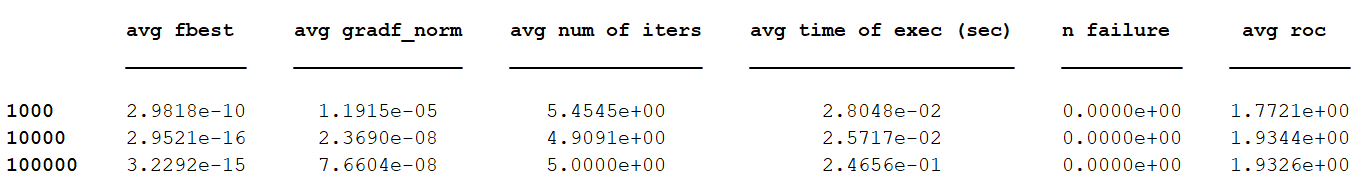
\includegraphics[width = 0.9\textwidth]{img/pb76_table_MN.png}
    \caption{Resultats obtained by running the Modified Newton Method on the problem $76$ using the exact derivatives.}
\end{figure*}

This time, the method always converges to the minimum point in very few iterations, even for higher dimensionalities. 
We can also appreciate the fact that the approximated rate of convergence is close to $2$, as expected for a Newton method.
Comparing this table with the previous one (showing the results obtained by running the symplex method), we can see that the Modified Newton method identifies as minimum a point in which the evaluation of the function is much smaller. 
This behavior aligns with theoretical expectations, as the Modified Newton method leverages the exact derivatives of the function $F(\mathbf{x})$ to determine the descent direction, while the symplex method depends only on function evaluations.

\medskip
\subsection*{Modified Newton Method - Approximated Derivatives}
Approximating the derivatives of the function $F(\mathbf{x})$ using finite differences is more challenging than it appears due to potential numerical cancellation issues, which can occur when subtracting two nearly equal quantities. Additionally, we aim to derive a formula that minimizes computational cost.

Let's begin by approximating the first-order derivatives of the function $F(\mathbf{x})$ using the centered finite difference formula with step $h_k$. The subscript $k$ is specified because the following formula are valid both with a constant increment, $h_k = k$ for all $h = 1, \dots, n$, and with a specific increment $h_k = h |\hat{x}_k| \; k= 1, \dots, n$, where $\mathbf{\hat{x}}$ is the point at which we approximate the derivatives.
$$ \frac{\partial F }{\partial x_k} (\mathbf{x}) \approx \frac{F(\mathbf{x} + h_k \vec{e}_k) - F(\mathbf{x} - h_k \vec{e}_k)}{2h_k} = 
\frac{\sum_{i = 1}^{n} f_i(\mathbf{x} + h_k \vec{e}_k)^2 - \sum_{i = 1}^{n} f_i(\mathbf{x} - h_k \vec{e}_k)^2}{4h_k}$$
We can observe that each term $f_i^2$ only depends on $x_i$ and $x_{i+1}$, so $f_i(\mathbf{x} + h_k\vec{e}_k)^2 - f_i(\mathbf{x} - h_k\vec{e}_k)^2 = 0$ for all $i \neq k-1, k$ (or $i \neq 1,n$ if we are considering $k = 1$). 
This allows to simplify the formula, even in order to decrease the computational cost, as follows
$$\frac{\partial F }{\partial x_k} (\mathbf{x}) \approx  \frac{f_{k-1}(\mathbf{x} + h_k\vec{e}_k)^2 - f_{k-1}(\mathbf{x} - h_k\vec{e}_k)^2 + f_{k}(\mathbf{x} + h_k\vec{e}_k)^2 - f_{k}(\mathbf{x} - h_k\vec{e}_k)^2}{4h_k}  \quad 1 < k \leq n$$
$$\frac{\partial F }{\partial x_k} (\mathbf{x}) \approx  \frac{f_{n}(\mathbf{x} + h_k\vec{e}_k)^2 - f_{n}(\mathbf{x} - h_k\vec{e}_k)^2 + f_{k}(\mathbf{x} + h_k\vec{e}_k)^2 - f_{k}(\mathbf{x} - h_k\vec{e}_k)^2}{4h_k}  \quad k = 1$$
In order to avoid numerical cancellation, the numerator has been expanded obtaining the following formula
\begin{align*}
    \frac{\partial F }{\partial x_1} (\mathbf{x}) & \approx \frac{4h_k x_1 - 2/5 h_k x_2^2 - 4/5 h_k x_n x_1 + 8/100 h_k x_1 (x_1^2 + h_k^2)}{4h_k} \\
    \frac{\partial F }{\partial x_k} (\mathbf{x}) & \approx \frac{4h_k x_k - 2/5 h_k x_{k+1}^2 - 4/5 h_k x_{k-1} x_k + 8/100 h_k x_k (x_k^2 + h_k^2)}{4h_k} \\
    \frac{\partial F }{\partial x_n} (\mathbf{x}) & \approx \frac{4h_k x_n - 2/5 h_k x_{1}^2 - 4/5 h_k x_{n-1} x_n + 8/100 h_k x_n (x_n^2 + h_k^2)}{4h_k}
\end{align*}


We can now proceed to approximate the second order derivatives of the function $F(\mathbf{x})$ using the centered finite difference formula; this time we need to use two different increments $h_i$ and $h_j$ based on the two components with respect to which we are differentiating.
The general formula is the following
$$ \frac{\partial^2 F}{\partial x_i \partial x_j} (\mathbf{x})  = \frac{F(\mathbf{x} + h_i \vec{e}_i + h_j \vec{e}_j) - F(\mathbf{x} + h_i \vec{e}_i) - F(\mathbf{x} - h_j \vec{e}_j) + F(\mathbf{x})}{h_i h_j}$$

The approximation of the Hessian matrix has to be approached taking into account its sparsity in order to reduce the computational cost, indeed in the Matlab script we have implemented a function that approximates the Hessian matrix just by computing the non-null terms which are the following
\begin{align*}
    & \frac{\partial^2 F}{\partial x_k^2} (\mathbf{x})  \approx 2h_k - \frac{2}{5} x_{k-1} h_k + \frac{12}{100} x_k^2 h_k^2 + \frac{24}{100}x_k h_k^3 + \frac{14}{100} h_k^2 \quad & 1 < k \leq n \\
    & \frac{\partial^2 F}{\partial x_k^2} (\mathbf{x})  \approx 2h_k - \frac{2}{5} x_{n} h_k + \frac{12}{100} x_k^2 h_k^2 + \frac{24}{100}x_k h_k^3 + \frac{14}{100} h_k^2 \quad  & k = 1 \\
    & \frac{\partial^2 F}{\partial x_k \partial x_{k+1}} (\mathbf{x})  \approx - \frac{2}{5} h_k h_{k+1} x_{k+1} - \frac{1}{5} h_k^2 h_{k+1} \quad & 1 \leq k < n 
\end{align*}
The values of the inferior diagonal are obtained by exploiting the symmetry of the Hessian matrix.

The terms have been computed following the same approach described above: the numerator has been expanded negletting the $f_i^2()$ that are not affected by the varation of the components with respect to which we are differentiating.


We now report some barplots showing the results obtained by running the Modified Newton method on the function $F(\mathbf{x})$ using the approximated derivatives.

\begin{figure}[htbp]
    \centering
    % Prima immagine
    \begin{subfigure}[t]{0.45\textwidth}  % Larghezza del 45% del testo
        \centering
        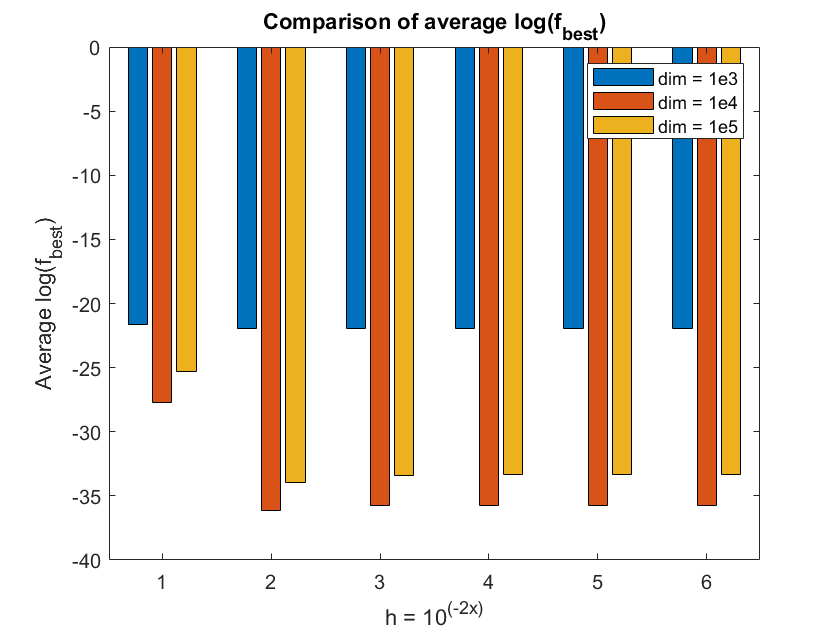
\includegraphics[width=\textwidth]{img/pb76_MN_difffinite_COST_log(fbest).png}
        \caption{Costant Increment $h$}
    \end{subfigure}
    \hspace{1cm} %spaziatura tra le immagini
    % Seconda immagine
    \begin{subfigure}[t]{0.45\textwidth}
        \centering
        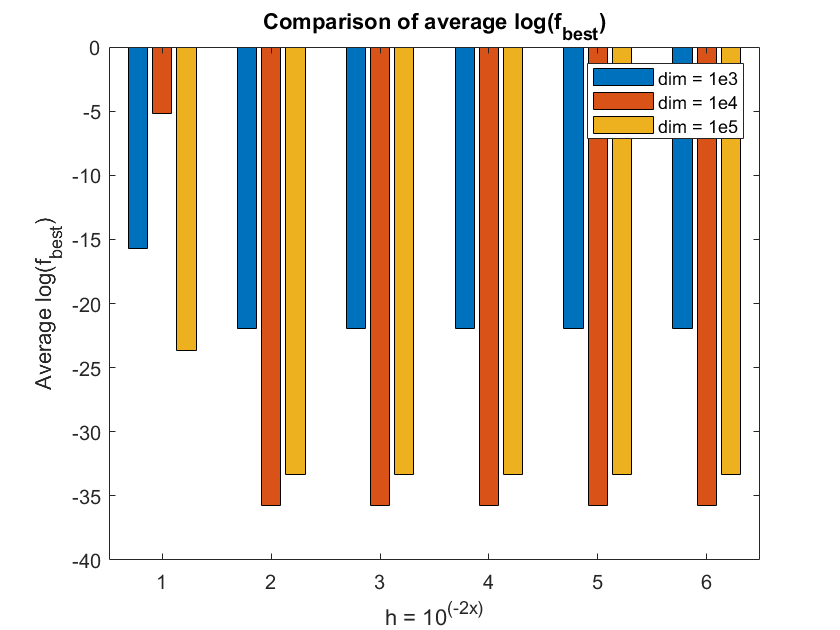
\includegraphics[width=\textwidth]{img/pb76_MN_difffinite_REL_log(fbest).png}
        \caption{Specific Increment }
    \end{subfigure}
    % Didascalia generale
    \caption{ \small Values of the average $\log(f_{best})$ in function of the increment while running the Modified Newton Method with approximated derivatives on the problem $76$.}
    \label{logfbest_difffinite76}
\end{figure}

As we can see from the plots $\eqref{logfbest_difffinite76}$, expecially for larger values of the increments, the algorithm converges to a point such that the value of the function is higher accordingly to the fact that the approximated derivatives are less accurate. Nonetheless, the method succeeds to find an acceptable approximation of the minimum value even when computing the descent direction with just an approximation of the derivatives.

\begin{figure*}[htbp]
    \centering
    % Prima immagine
    \begin{subfigure}[t]{0.45\textwidth}  % Larghezza del 45% del testo
        \centering
        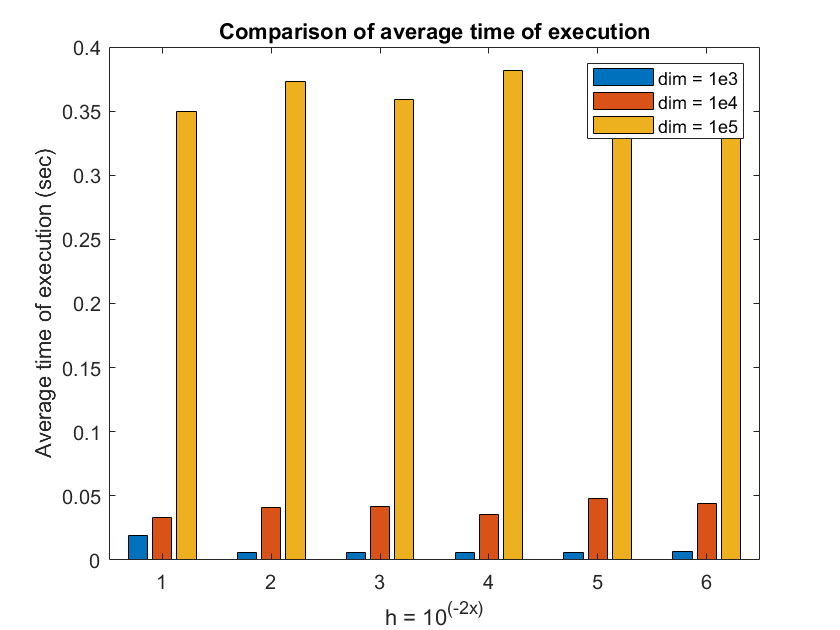
\includegraphics[width=\textwidth]{img/pb76_MN_difffinite_COST_timeofexec.png}
        \caption{Costant Increment $h$}
    \end{subfigure}
    \hspace{1cm} %spaziatura tra le immagini
    % Seconda immagine
    \begin{subfigure}[t]{0.45\textwidth}
        \centering
        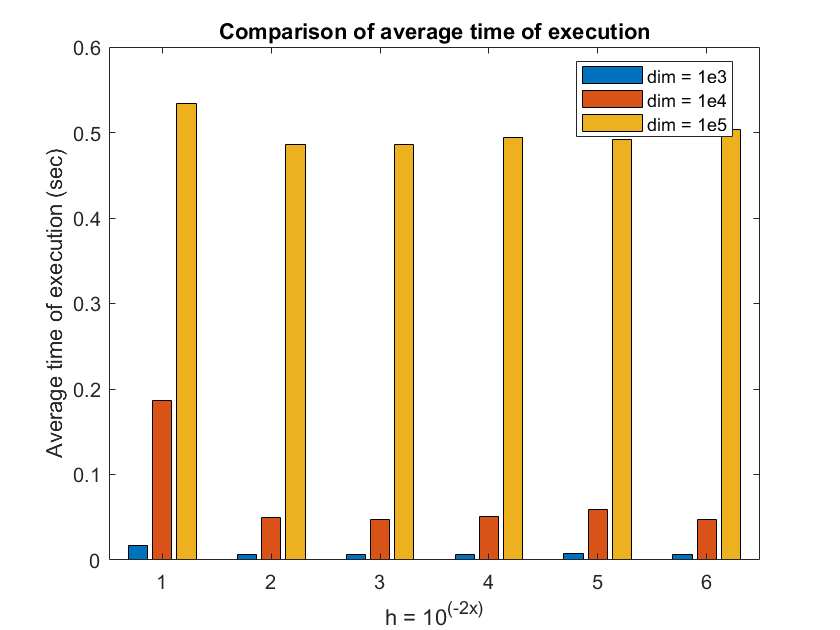
\includegraphics[width=\textwidth]{img/pb76_MN_difffinite_REL_timeofexec.png}
        \caption{Specific Increment }
    \end{subfigure}
    % Didascalia generale
    \caption{ \small Average time of execution in function of the increment $h$  while running the Modified Newton Method with approximated derivatives on the problem $76$.}
\end{figure*}


\begin{figure*}[htbp]
    \centering
    % Prima immagine
    \begin{subfigure}[t]{0.45\textwidth}  % Larghezza del 45% del testo
        \centering
        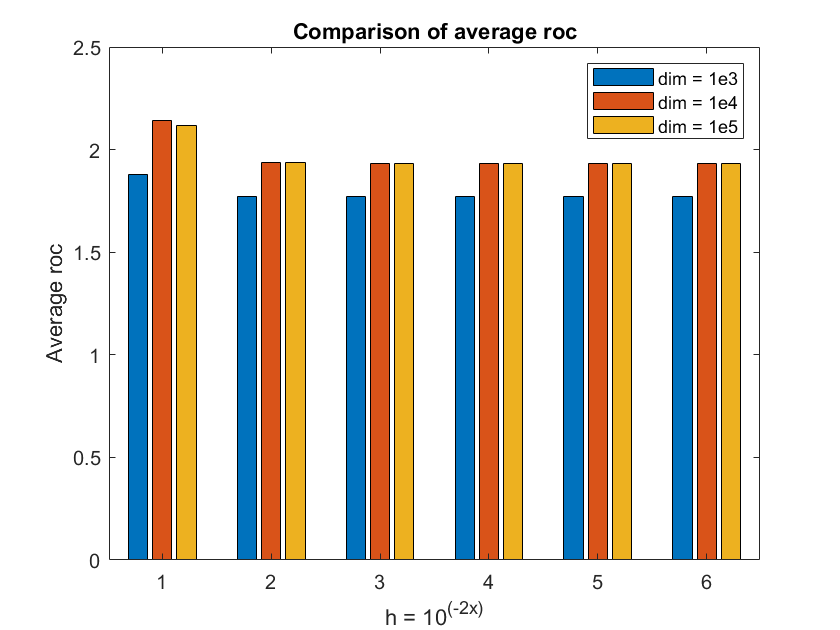
\includegraphics[width=\textwidth]{img/pb76_MN_difffinite_COST_rateofconv.png}
        \caption{Costant Increment $h$}
    \end{subfigure}
    \hspace{1cm} %spaziatura tra le immagini
    % Seconda immagine
    \begin{subfigure}[t]{0.45\textwidth}
        \centering
        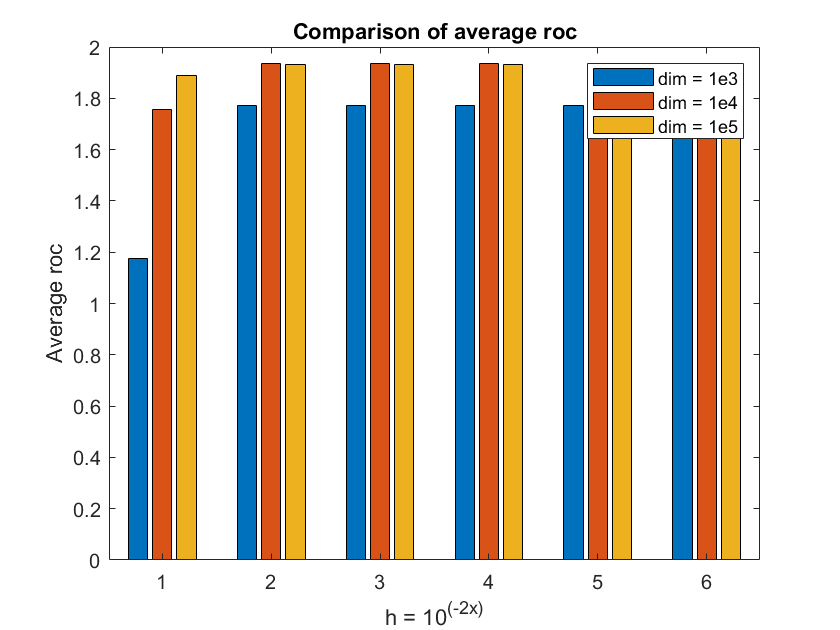
\includegraphics[width=\textwidth]{img/pb76_MN_difffinite_REL_rateofconv.png}
        \caption{Specific Increment }
    \end{subfigure}
    % Didascalia generale
    \caption{ \small Average values of the experimental rate of convergence in function of the increment $h$  while running the Modified Newton Method with approximated derivatives on the problem $76$.}
\end{figure*}


The others plots show that the average time of execution and the average rate of convergence are not significantly affected by the approximation of the derivatives for none of the values oh the increment $h$.

\newpage
\section*{CONCLUSIONI}
Summarizing the results obtained by exploiting Nelder Mead and Modified Newton methods for 
unconstrained optimization of the considered functions, we can say that, as expected, the 
simplex methods performs more poorly (even considering that the dimensionalities we tested it 
on were significantly smaller than those used for the Modified Newton). This happens because 
we are using a black box method on some problems that have high regularity, so the choice is 
not optimal because it does not exploit a lot of useful information coming from the derivatives. 
However, even if it does not always find the true minimizer, it is usually able to return a solution 
that is not so far away from it.

Modified Newton method using exact derivatives is, as expected, the best choice in all considered cases. 
Exploiting the derivatives it is able to always find the minimizer even when the function presents 
some flat areas.

When using the approximation of derivatives, we saw that the shape of the function greatly influences the 
succeed of the method: when flat areas are present, more problems arise. Also, the choice of the increment 
$h_k$ influences the possibility of success, but the best choice for this value is not always the same 
and should be chosen after some testings on the specific problem.



\end{document}